%%=============================================================================
%% Methodologie
%%=============================================================================

\chapter{\IfLanguageName{dutch}{Methodologie}{Methodology}}%
\label{ch:methodologie}

Dit onderzoek wordt uitgevoerd in verschillende fasen, waarbij elke fase een specifieke doelstelling heeft en resulteert in concrete deliverables. De gekozen aanpak is gebaseerd op een iteratieve en stapsgewijze ontwikkeling van een mobiele applicatie met \texttt{.NET MAUI}, waarbij zowel frontend als backendcomponenten worden ontwikkeld en getest. In dit hoofdstuk worden de verschillende fasen toegelicht en wordt verantwoord waarom deze aanpak is gekozen.

\section{Omgeving klaarzetten}

De eerste stap in het onderzoek is het opzetten van de ontwikkelomgeving. Dit is noodzakelijk om een stabiele en efficiënte werkomgeving te creëren waarin de mobiele applicatie kan worden ontwikkeld en getest. Hiervoor wordt .NET MAUI als ontwikkelplatform geïnstalleerd en geconfigureerd. Daarnaast worden verschillende simulators opgezet om de applicatie op meerdere apparaten te testen.\\

De architectuur van het project wordt opgezet met een duidelijke scheiding van verantwoordelijkheden over verschillende lagen. Er wordt een API-laag opgezet waarin gebruik wordt gemaakt van controllers om de communicatie tussen de mobiele client en de backend mogelijk te maken. Binnen deze laag wordt gebruikgemaakt van entiteitmodellen voor de representatie van de databaseobjecten, migraties om de lokale database stapsgewijs op te bouwen, en services om de logica af te handelen.\\

Daarnaast wordt een Client-laag, genaamd ATS, ingericht waarin alle front-end gerelateerde onderdelen van de applicatie zijn ondergebracht. Deze laag bevat de Views (voor de UI-schermen), ViewModels (voor de logica en data-binding), en client-side services voor communicatie met de backend. \\

Om herbruikbaarheid en consistentie te bevorderen, wordt ook een aparte Shared-laag toegevoegd. Deze bevat gedeelde onderdelen zoals DTO's (Data Transfer Objects), Enums en Interfaces, die zowel door de backend als door de client kunnen worden gebruikt. Dit zorgt ervoor dat gegevensstructuren consistent blijven tussen beide zijden van de applicatie. \\

Tot slot wordt een database ingericht om gebruikersgegevens en authenticatie-informatie op te slaan. De gekozen methode voor deze fase bestaat uit het raadplegen van de officiële documentatie van .NET MAUI en het uitvoeren van praktische experimenten om de configuratie optimaal af te stemmen. Het resultaat van deze fase is een volledig geconfigureerde ontwikkelomgeving, inclusief de benodigde tools, frameworks, projectstructuur en databases.\\

\begin{figure}[H]
	\centering
	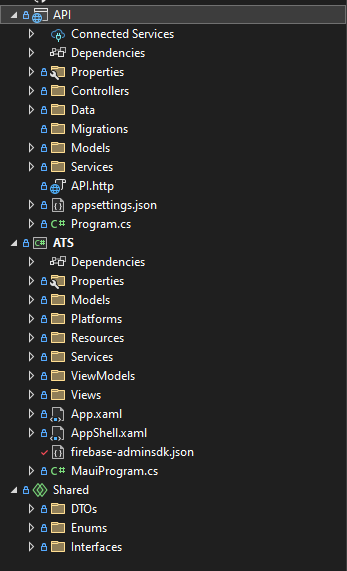
\includegraphics[scale=0.5]{omgeving.png}
	\caption{Werkomgeving van het project}
	\label{fig:omgeving}
\end{figure}

\section{Loginpagina}

In de tweede fase wordt de basisfunctionaliteit voor gebruikersauthenticatie geïmplementeerd. De focus ligt op het ontwerpen en ontwikkelen van een gebruiksvriendelijke loginpagina. Hiervoor wordt eerst de frontend ontwikkeld in .NET MAUI(XAML-code), waarbij gebruik wordt gemaakt van standaard UI-componenten en best practices op het gebied van gebruiksvriendelijkheid. \\

\begin{figure}[H]
	\centering
	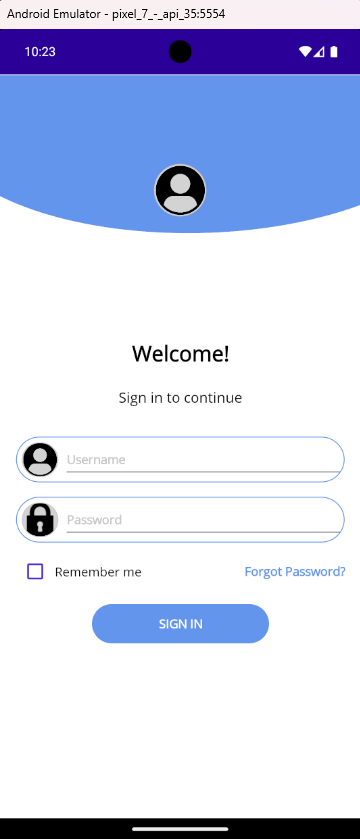
\includegraphics[scale=0.5]{login.png}
	\caption{Loginpagina ontworpen in .NET MAUI}
	\label{fig:loginpagina}
\end{figure}

Vervolgens wordt een backend opgezet waarin gebruikersgegevens worden beheerd en gecontroleerd via een database. Na de implementatie wordt de loginpagina getest op verschillende apparaten om de correcte werking te garanderen. Tijdens deze fase wordt gebruikgemaakt van officiële documentatie en technische bronnen om de implementatie te ondersteunen. Verschillende oplossingen worden onderzocht, toegepast en geëvalueerd om tot een stabiele en veilige authenticatieoplossing te komen. Het eindresultaat is een werkende loginpagina die correct communiceert met de backend en gebruikersgegevens valideert.

\begin{figure}[H]
	\centering
	\includegraphics[width=0.6\textwidth]{gebruikerstabel.png}
	\caption{Succesvol toevoegen van gebruikers in lokale database}
	\label{fig:gebruikerstabel}
\end{figure}

\section{JWT Authenticatie en Hashing}

De derde fase richt zich op het beveiligen van de gebruikersauthenticatie door middel van JWT (JSON Web Token) en hashing-technieken. Dit is een cruciale stap om ongeautoriseerde toegang te voorkomen en gebruikersgegevens veilig op te slaan. JWT wordt geïmplementeerd als mechanisme voor sessiebeheer, waarbij gebruikers een token ontvangen na succesvolle authenticatie. Dit token wordt vervolgens gebruikt om toegang te krijgen tot beveiligde endpoints. Daarnaast worden wachtwoorden gehasht opgeslagen in de database, zodat ze niet in platte tekst beschikbaar zijn. De beveiligingsmechanismen worden uitvoerig getest om mogelijke zwakke plekken te identificeren en te verbeteren. \\

\begin{figure}[H]
	\centering
	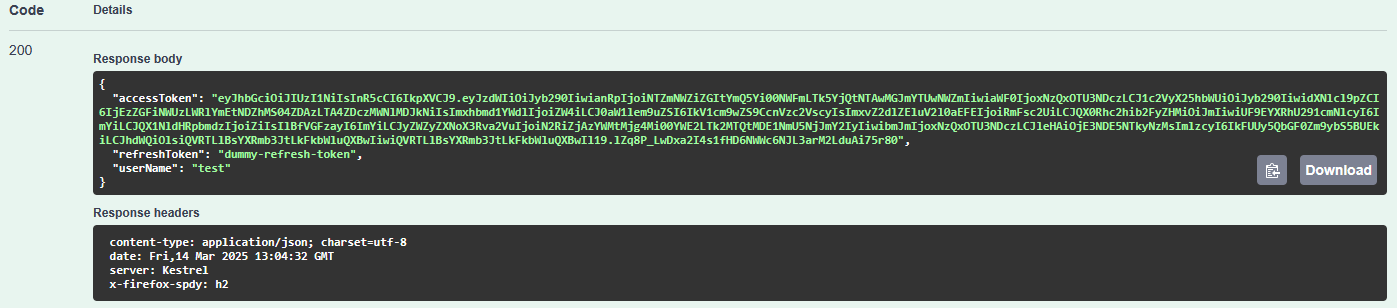
\includegraphics[scale=0.5]{token.png}
	\caption{Token na een succesvolle login met info over gebruiker}
	\label{fig:token}
\end{figure}

Het resultaat is een veilige en betrouwbare loginomgeving die voldoet aan moderne beveiligingsstandaarden. Om het sessiebeheer verder te versterken, wordt ervoor gekozen om het JWT-token niet op te slaan in een lokale database, maar in de secure storage van het mobiele besturingssysteem. Deze opslaglocatie is speciaal ontworpen voor het veilig bewaren van gevoelige informatie en biedt verhoogde bescherming tegen ongeautoriseerde toegang of reverse engineering van de applicatie. Een bijkomend voordeel van deze aanpak is dat het token automatisch beschikbaar blijft zolang de gebruiker is aangemeld, zonder dat een externe databank geconsulteerd hoeft te worden. Bij uitloggen wordt het token expliciet verwijderd, waardoor de toegang volledig wordt afgesloten. Deze methode sluit goed aan bij de vereisten van mobiele applicatiebeveiliging en verhoogt zowel de gebruiksvriendelijkheid als de veiligheid van de app.

\section{Pushnotificaties}

In deze fase wordt de mogelijkheid toegevoegd om pushnotificaties te ontvangen en te verzenden binnen de mobiele applicatie. Het doel hiervan is om gebruikers automatisch op de hoogte te brengen van belangrijke updates, bijvoorbeeld wanneer hun systeem een overschot aan zonne-energie detecteert. Om dit te realiseren, wordt de applicatie zodanig ingesteld dat elk toestel een unieke code (token) ontvangt zodra de app wordt geopend. Deze token wordt vervolgens gekoppeld aan de juiste gebruiker, zodat meldingen persoonlijk en correct afgeleverd kunnen worden.

Daarnaast wordt ervoor gezorgd dat de app, wanneer er op een melding wordt geklikt, automatisch naar de juiste pagina navigeert. Dit is belangrijk omdat gebruikers zo direct toegang krijgen tot de relevante informatie zonder handmatig door de applicatie te moeten zoeken.

Voor het testen van de pushnotificaties wordt gebruikgemaakt van het platform Postman. Hiermee kunnen handmatig HTTP-verzoeken naar Firebase worden gestuurd, waarmee notificaties naar specifieke toestellen worden verzonden. Dit laat toe om de correcte werking van de Firebase-configuratie te controleren, nog vóór de volledige applicatie is geïntegreerd. Bovendien biedt deze aanpak de mogelijkheid om meldingen te testen op meerdere apparaten – iets wat met een enkele emulator moeilijk te realiseren is. Door Postman als testtool in te zetten, kan het notificatiesysteem grondig en efficiënt gevalideerd worden.

Tot slot wordt de algemene werking getest op verschillende toestellen en wordt gecontroleerd of de notificaties ook aankomen wanneer de app niet actief is. Deze aanpak zorgt ervoor dat de meldingen betrouwbaar en gebruiksvriendelijk functioneren binnen de volledige gebruikerservaring. \\

\begin{figure}[H]
	\centering
	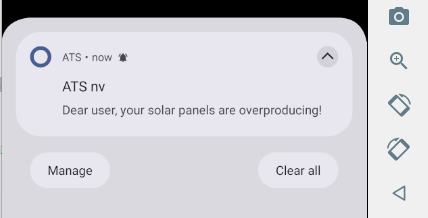
\includegraphics[width=0.6\textwidth]{notification.png}
	\caption{Het succesvol ontvangen van een notificatie}
	\label{fig:notification}
\end{figure}

\section{Resultaten en Integratie}

Nu de verschillende technologieën en technieken succesvol getest zijn in een kleiner, losstaand project, kan worden besloten dat ze in principe goed werken. Denk hierbij aan zaken zoals JWT-authenticatie, veilige opslag van tokens en pushnotificaties via Firebase. De testresultaten zijn positief en tonen aan dat deze methodes technisch haalbaar zijn en ook goed functioneren binnen een mobiele applicatie.

Hoewel alles in deze bachelorproef is opgebouwd en getest in een aparte proof of concept, is het de bedoeling dat deze aanpak op termijn wordt geïntegreerd in SmartKit, de bestaande tool van het bedrijf. Binnen de scope van dit onderzoek ligt de focus echter op het uitvoeren van een verkennend onderzoek en het ontwikkelen van een eerste concept. Een volledige integratie in SmartKit zelf zit dus niet in de opdracht, aangezien dat meer tijd, afstemming en grondige testing vraagt.

Toch tonen de behaalde resultaten aan dat de implementatie van deze technologieën in SmartKit zeker mogelijk is en ook een duidelijke meerwaarde zou kunnen bieden. Het vormt dan ook een goede basis voor verdere ontwikkeling en integratie in de toekomst.
